\documentclass[aspectratio=169]{beamer}
\usetheme{CambridgeUS}
\usecolortheme{dolphin}
\usepackage{graphicx}
\usepackage{booktabs}
\usepackage{tikz}

% Remove navigation symbols
\setbeamertemplate{navigation symbols}{}

% Add slide numbers
\setbeamertemplate{footline}[frame number]

\title{Fast Failure Recovery in Distributed Training\\with In-Memory Checkpoints}
\subtitle{Gemini Reproduction Study — CS240 Fall 2025}
\author{Mustafa Albahrani \and Mohammed Alkhalifah}
\institute{King Abdullah University of Science and Technology}
\date{}

\begin{document}

% ============================================
% SLIDE 1: Title
% ============================================
\begin{frame}
\titlepage
\end{frame}

% ============================================
% SLIDE 2: Motivation - The Problem
% ============================================
\begin{frame}{The Problem: Failures in Large-Scale Training}

\begin{columns}
\begin{column}{0.55\textwidth}
\textbf{Modern AI training is failure-prone:}
\begin{itemize}
    \item Training runs span \textbf{days to weeks}
    \item Thousands of GPUs = hardware failures inevitable
    \item \textbf{Traditional solution:} Checkpoint to disk (NFS)
\end{itemize}

\vspace{0.5cm}
\textbf{The cost of disk checkpointing:}
\begin{itemize}
    \item Slow writes (seconds to minutes)
    \item Training blocked during I/O
    \item Recovery requires full reload from disk
    \item \alert{Wasted GPU-hours = wasted money}
\end{itemize}
\end{column}

\begin{column}{0.45\textwidth}
\begin{center}
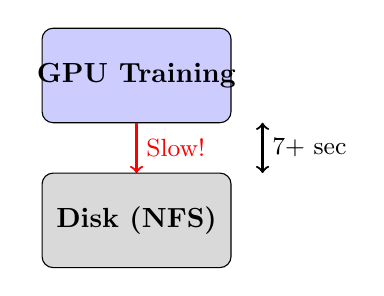
\begin{tikzpicture}[scale=0.8]
    % GPU box
    \draw[fill=blue!20, rounded corners] (0,0) rectangle (3,1.5);
    \node at (1.5, 0.75) {\textbf{GPU Training}};
    
    % Arrow down
    \draw[->, thick, red] (1.5, 0) -- (1.5, -0.8);
    \node[red, right] at (1.5, -0.4) {\small Slow!};
    
    % Disk
    \draw[fill=gray!30, rounded corners] (0,-2.3) rectangle (3,-0.8);
    \node at (1.5, -1.55) {\textbf{Disk (NFS)}};
    
    % Time indicator
    \draw[<->, thick] (3.5, 0) -- (3.5, -0.8);
    \node[right] at (3.5, -0.4) {\small 7+ sec};
\end{tikzpicture}
\end{center}
\end{column}
\end{columns}

\end{frame}

% ============================================
% SLIDE 3: Gemini Solution
% ============================================
\begin{frame}{The Gemini Solution (SOSP 2023)}

\textbf{Key insight:} RAM is 100× faster than disk — use it for checkpoints!

\vspace{0.3cm}
\begin{columns}
\begin{column}{0.5\textwidth}
\textbf{Gemini's approach:}
\begin{enumerate}
    \item Store checkpoints in \textbf{CPU RAM}
    \item Replicate to peer nodes for fault tolerance
    \item On failure: recover from RAM, not disk
\end{enumerate}

\vspace{0.3cm}
\textbf{Paper's setup \& results:}
\begin{itemize}
    \item 128× A100 GPUs (16 AWS p4d.24xlarge)
    \item Models: GPT-2, BERT, RoBERTa (up to 100B)
    \item $>$13× faster recovery, 92\% less waste
\end{itemize}
\end{column}

\begin{column}{0.5\textwidth}
\begin{center}
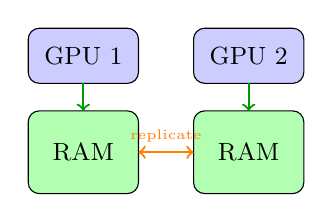
\begin{tikzpicture}[scale=0.7]
    % GPU 1
    \draw[fill=blue!20, rounded corners] (0,2) rectangle (2,3);
    \node at (1, 2.5) {\small GPU 1};
    
    % GPU 2
    \draw[fill=blue!20, rounded corners] (3,2) rectangle (5,3);
    \node at (4, 2.5) {\small GPU 2};
    
    % RAM 1
    \draw[fill=green!30, rounded corners] (0,0) rectangle (2,1.5);
    \node at (1, 0.75) {\small RAM};
    
    % RAM 2
    \draw[fill=green!30, rounded corners] (3,0) rectangle (5,1.5);
    \node at (4, 0.75) {\small RAM};
    
    % Arrows
    \draw[->, thick, green!60!black] (1, 2) -- (1, 1.5);
    \draw[->, thick, green!60!black] (4, 2) -- (4, 1.5);
    
    % Replication arrow
    \draw[<->, thick, orange] (2, 0.75) -- (3, 0.75);
    \node[above, orange] at (2.5, 0.75) {\tiny replicate};
\end{tikzpicture}
\end{center}
\end{column}
\end{columns}

\vspace{0.3cm}
\textbf{Our goal:} Reproduce these results on 4× A100 GPUs

\end{frame}

% ============================================
% SLIDE 4: What We Built
% ============================================
\begin{frame}{What We Built}

\begin{columns}
\begin{column}{0.5\textwidth}
\textbf{Implementation components:}
\begin{enumerate}
    \item \textbf{Baseline trainer}\\
    {\small DDP + disk checkpointing}
    
    \vspace{0.2cm}
    \item \textbf{In-memory checkpoint manager}\\
    {\small RAM-based saves using BytesIO}
    
    \vspace{0.2cm}
    \item \textbf{Replication manager}\\
    {\small Ring topology: GPU$_i$ → GPU$_{i+1}$}
    
    \vspace{0.2cm}
    \item \textbf{Failure simulation}\\
    {\small Application-level injection}
\end{enumerate}
\end{column}

\begin{column}{0.5\textwidth}
\textbf{Experimental setup:}
\begin{itemize}
    \item \textbf{Hardware:} 4× NVIDIA A100 (Vast.ai)
    \item \textbf{Framework:} PyTorch 2.8, CUDA 12.9
    \item \textbf{Model:} 12-layer Transformer\\
    {\small (1024 hidden, 16 heads, ~630M params)}
    \item \textbf{Runs:} 3 runs, 100 iterations each
    \item \textbf{Checkpoints:} Every 25 iterations
\end{itemize}
\end{column}
\end{columns}

\end{frame}

% ============================================
% SLIDE 5: Results - Checkpoint Speedup
% ============================================
\begin{frame}{Results: Checkpoint Time}

\begin{columns}
\begin{column}{0.5\textwidth}
\includegraphics[width=\textwidth]{figures/fig1_checkpoint_time.png}
\end{column}

\begin{column}{0.5\textwidth}
\textbf{Single-GPU checkpoint save:}
\begin{itemize}
    \item Disk: 7,012 ms
    \item RAM: 512 ms
    \item \textbf{Speedup: 13.7×} ✓
\end{itemize}

\vspace{0.5cm}
\textbf{Why faster?}
\begin{itemize}
    \item No disk I/O bottleneck
    \item Direct memory serialization
    \item No filesystem overhead
\end{itemize}

\vspace{0.3cm}
\alert{Matches paper's $>$13× claim!}
\end{column}
\end{columns}

\end{frame}

% ============================================
% SLIDE 6: Results - All Speedups
% ============================================
\begin{frame}{Results: Overall Speedups}

\begin{columns}
\begin{column}{0.55\textwidth}
\includegraphics[width=\textwidth]{figures/fig5_speedup_summary.png}
\end{column}

\begin{column}{0.45\textwidth}
\begin{table}
\small
\begin{tabular}{@{}lrr@{}}
\toprule
\textbf{Metric} & \textbf{Ours} & \textbf{Paper} \\
\midrule
Checkpoint & 13.7× & $>$13× \\
Recovery & 6.1× & $>$13× \\
Multi-GPU rec. & 4.6× & — \\
Throughput & +100\% & minimal \\
\bottomrule
\end{tabular}
\end{table}

\vspace{0.3cm}
\textbf{Key observations:}
\begin{itemize}
    \item Checkpoint: \textcolor{green!60!black}{\textbf{matches paper}}
    \item Recovery: below paper (expected)
    \item Throughput: \textbf{2× improvement!}
\end{itemize}
\end{column}
\end{columns}

\end{frame}

% ============================================
% SLIDE 7: Analysis & Limitations
% ============================================
\begin{frame}{Analysis: Why Recovery is Slower Than Paper}

\textbf{Our recovery speedup: 6.1× \hspace{1cm} Paper: $>$13×}

\vspace{0.3cm}
\begin{columns}
\begin{column}{0.5\textwidth}
\textbf{Reasons for the gap:}
\begin{enumerate}
    \item \textbf{Scale difference}\\
    {\small Paper: 128 A100s (AWS p4d.24xlarge)\\
    Ours: 4 A100s (Vast.ai)}
    
    \vspace{0.2cm}
    \item \textbf{Model size}\\
    {\small Paper: up to 100B parameters\\
    Ours: ~630M parameters}
    
    \vspace{0.2cm}
    \item \textbf{Failure simulation}\\
    {\small Paper: real process kills\\
    Ours: application-level}
\end{enumerate}
\end{column}

\begin{column}{0.5\textwidth}
\textbf{Limitations:}
\begin{itemize}
    \item Memory overhead: ~1.9 GB/checkpoint
    \item Single-node replication only
    \item No real distributed failure testing
\end{itemize}

\vspace{0.3cm}
\textbf{What worked well:}
\begin{itemize}
    \item ✓ Core checkpoint speedup reproduced
    \item ✓ Throughput improved (not just maintained)
    \item ✓ Modular, testable implementation
\end{itemize}
\end{column}
\end{columns}

\end{frame}

% ============================================
% SLIDE 8: Conclusions
% ============================================
\begin{frame}{Conclusions}

\begin{columns}
\begin{column}{0.6\textwidth}
\textbf{We successfully reproduced Gemini's core claim:}
\begin{itemize}
    \item \textbf{13.7× faster checkpoints} (paper: $>$13×) ✓
    \item \textbf{6.1× faster recovery} (paper: $>$13×) ✗
    \item \textbf{+100\% throughput} (paper: minimal overhead) ✓
\end{itemize}

\vspace{0.5cm}
\textbf{Key takeaways:}
\begin{itemize}
    \item In-memory checkpointing is \textbf{practical}
    \item Even small-scale tests show \textbf{significant gains}
    \item Recovery benefits increase with cluster size
\end{itemize}
\end{column}

\begin{column}{0.4\textwidth}
\textbf{Future work:}
\begin{itemize}
    \item Scale to 16–64 GPUs
    \item Real failure injection (SIGKILL)
    \item Production models (GPT-2)
    \item Checkpoint compression
\end{itemize}

\vspace{0.5cm}
\begin{center}
\Large\textbf{Questions?}
\end{center}
\end{column}
\end{columns}

\vspace{0.5cm}
\begin{center}
\small Code: \texttt{github.com/Mustbhr/CS240-Project}
\end{center}

\end{frame}

\end{document}
